\section{GROUP THEORY}
\subsection{Group Definition}
A \textbf{Group} G, is a set with a rule for assigning to every (ordered) pair of
elements, a third element, satisfying:

1. If f, g $\epsilon$ G then h = fg $\epsilon$ G. \\
2. Associativity: $\forall$ f, g, h $\epsilon$ G, f(gh) = (fg)h. \\
3. Existence of identity element: $\forall$ f $\epsilon$ G $\exists$ \textit{e} s.t. \textit{e}f = f\textit{e} = f. \\
4. Existence of inverse element: $\forall$ f $\epsilon$ G $\exists$ f $^{-1}$ s.t. f f$^{-1}$ = f$^{-1}$f = \textit{e}.
\begin{figure}[h]
    \centering
    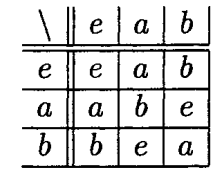
\includegraphics[width=0.3\textwidth]{figures/z3-group.png}
    \caption{Z$_3$ group multiplication table. (Every row and column
    of the multiplication table contains each element of the group exactly once.
    This must be the case because the inverse exists.)}
\end{figure}

A group G is \textbf{finite} if it has a finite number of elements. Otherwise it is \textbf{infinite}.
The number of elements in a finite group G is called the \textbf{order} of G. For eg: Z$_3$, the cyclic group of order 3.

An \textbf{Abelian group} G in one in which the multiplication law is commutative i.e.
g$_1$g$_2$ = g$_2$g$_1$. And the one which doesn't follows commutation is called \textbf{non-Abelian group}.

\subsection{Representation}
A \textbf{Representation} of a group G is a mapping D of the elements of G onto a set of
linear operators with the following properties:

1. D(\textit{e}) = 1, where 1 is the identity operator in the space on which
the linear operators act. \\
2. D(g$_1$)D(g$_2$) = D(g$_1$g$_2$) i.e. the group multiplication law 
is mapped onto the natural multiplication in the linear space on which the linear operators act.

For eg: representation of Z$_3$ is,
\begin{equation}
    D(e) = 1, \hspace{1cm} D(a) = e^{2\pi i/3}, \hspace{1cm} D(b) = e^{4\pi i/3}
\end{equation}
another representation of Z$_3$ can be directly constructed from the multiplication table as,
\begin{equation}
    D(e) = \begin{pmatrix}
        1 & 0 & 0 \\ 
        0 & 1 & 0 \\ 
        0 & 0 & 1 \\ 
   \end{pmatrix}, \hspace{1cm} 
   D(a) = \begin{pmatrix}
        0 & 0 & 1 \\ 
        1 & 0 & 0 \\ 
        0 & 1 & 0 \\ 
   \end{pmatrix}, \hspace{1cm} 
   D(b) = \begin{pmatrix}
        0 & 1 & 0 \\ 
        0 & 1 & 1 \\ 
        1 & 0 & 0 \\ 
\end{pmatrix},
\end{equation}

By taking the group elements themselves to form an orthonormal basis for a vector space, 
$|e \rangle$, $|a\rangle$, and $|b\rangle$ we can also define \textbf{regular representation} as,
\begin{equation}
    D(g_1)|g_2\rangle = |g_1g_2\rangle
    \label{eqn:representation}
\end{equation}

The \textbf{dimension of a representation} is the dimension of the space on which
it acts and the dimension of the regular representation is the order of the group. The representation of Z$_3$ is 1 dimensional.
For any finite group, we can define a vector space in which the basis vectors are labeled by the group elements.
Then equation \ref{eqn:representation} defines the regular representation.

\subsection{Subgroup}
A group H whose elements are all elements of a group G is called a subgroup of G. 
The identity, and the group G are trivial subgroups of G. For eg., the permutation group S3, has a Z3 subgroup formed by the elements \{e, a$_1$, a$_2$\}. 
Subgroup can be used to divide up the elements of the group into subsets called \href{https://en.wikipedia.org/wiki/Coset}{\textbf{cosets}}.
Given an element \textit{g} of G, the \textbf{left cosets} of H in G are the sets obtained by multiplying each element of H by a fixed element \textit{g} of G (where \textit{g} is the \textbf{left factor})
\begin{center}
    \textit{g}H = \{\textit{g}h : h $\epsilon$ H\} $\forall$ \textit{g} $\epsilon$ G.
\end{center}
The \textbf{right cosets} can be defined similarly where g is now a \textbf{right factor}.
\begin{center}
    H\textit{g} = \{h\textit{g} : h $\epsilon$ H\} $\forall$ \textit{g} $\epsilon$ G.
\end{center}

The number of elements in each coset is the order of H. Every element of G
must belong to one and only one coset. Thus for finite groups, the order of
a subgroup H must be a factor of order of G. 
A subgroup H of G is called an \textbf{invariant} or \textbf{normal subgroup} if $\forall$ g$\epsilon$G
\begin{equation}
    gH = Hg
\end{equation}

i.e.$\forall$ \textit{g} $\epsilon$G and \textit{h}$_1 \: \epsilon$ H $\exists$ an \textit{h}$_2 \: \epsilon$ H s.t.
\begin{center}
    \textit{h}$_1$\textit{g} = \textit{gh}$_2$, or \textit{gh}$_2$\textit{g}$^{-1}$ = \textit{h}$_2$.
\end{center} 

The trivial subgroups e and G are invariant for any group. If H is invariant then H\textit{g}$_1$ H\textit{g}$_1^{-1}$ = H, 
so the product of elements in two cosets is in the coset represented by the product of the elements. 
In this case, the coset space G/H, is called the \textbf{factor group} of G by H.

The \textbf{center} of a group G is the set of all elements of G that commute
with all elements of G. The center is always an Abelian, invariant subgroup
of G. However, it may be trivial, consisting only of the identity, or of the
whole group.

The \textbf{characters} $\chi_D$(g) of a group representation D are the traces of the linear
operators of the representation or their matrix elements:
\begin{equation}
    \chi_D(g) \equiv Tr D(g) = \sum_{i}[D(g)]_{ii}
\end{equation}

The advantage of the characters is that because of the cyclic property of the trace Tr(AB) = Tr(BA), they are unchanged by similarity transformations,
thus all equivalent representations have the same characters. The characters are also different for each inequivalent irreducible representation, D$_a$\textemdash 
in fact, they are orthonormal up to an overall factor of N.

\subsection{Eigenstates}
In quantum mechanics, we are often interested in the eigenstates of an invariant hermitian operator, in particular the Hamiltonian, H. 
We can always take these eigenstates to transform according to irreducible representations of the symmetry group. 
To prove this, note that we can divide up the Hilbert space into subspaces with different eigenvalues of H. 
Each subspace furnishes a representation of the symmetry group because D(\textit{g}), the group representation on the full Hilbert space, 
cannot change the H eigenvalue because [D(\textit{g}), H] = 0. But then we can completely reduce the representation in each subspace.
If some irreducible representation appears only once in the Hilbert space, then the states in that representation must be eigenstates
of H (and any other invariant operator). This is true because H$|a, j, x\rangle$ must be in the same irreducible representation, thus
\begin{equation}
    H|a, j, x\rangle = \sum_{y} c_y |a, j, x\rangle
\end{equation}
and if x andy take only one value, then $|a, j, x\rangle$ is an eigenstate.

\textbf{Theorem:} If a hermitian operator H, commutes with all the elements D(\textit{g}), of a representation of the group G, 
then you can choose the eigenstates of H to transform according to irreducible representations of G. 
If an irreducible representation appears only once in the Hilbert space, every state in the irreducible representation 
is an eigenstate of H with the same eigenvalue.

For Abelian groups, this procedure of choosing the H eigenstates to transform under irreducible representations is analogous to simultaneously 
diagonalizing H and D(\textit{g}) because for an Abelian group that commutes with the H, the group elements can simultaneously
diagonalized along with H. This is a consequence of theorem,

\textbf{Theorem:} All of the irreducible representations of a finite Abelian group are 1-dimensional.

For a non-Abelian group, we cannot simultaneously diagonalize all of the D(\textit{g})s, 
but we can completely reduce the representation on each subspace of constant H.
A classical problem which is quite analogous to the problem of diagonalizing the Hamiltonian  in quantum mechanics 
is the problem of finding the normal modes of small oscillations of a mechanical system about a point of stable equilibrium. 
Here, the square of the angular frequency is the eigenvalue of the M$^{-1}$K matrix and the normal modes are the eigenvectors of M$^{-1}$K.

\subsection{Tensor Product Representation}
Suppose that D$_1$ is an m-dimensional representation acting on a space with basis vectors $|j\rangle$ for j = 1 to m and 
D$_2$ is an n-dimensional representation acting on a space with basis vectors $|x\rangle$ for x = 1 to n. 
We can make an m $\times$ n dimensional space called the \textbf{tensor product space} by taking basis vectors labeled by both j and x  in an ordered pair $|j, x\rangle$. 
Then when j goes from 1 to m and x goes from 1 to n, the ordered pair (j, x) runs over m $\times$ n different combinations. 
On this product space, we can define a new representation called the \textbf{tensor product representation} D$_1 \otimes$D$_2$ by multiplying the two smaller representations. 
More precisely, the matrix elements of D$_{D_1 \otimes D_2}$(\textit{g}) are products of those of D$_1$(\textit{g}) and D$_2$(\textit{g}):
\begin{equation}
    \langle j, x| D_{D_1 \otimes D_2}(g)|k, y \rangle \equiv \langle j| D_1(g)|k \rangle \langle x|D_2(g)|y \rangle
\end{equation}

\subsection{Symmetry Group \texorpdfstring{S$_n$}. (Permutation Group)}
A permutation group is a group G whose elements are permutations of a given set M and whose group operation is the composition of permutations in G.
The group of all permutations of a set M is the symmetric group of M, often written as Sym(M) or S$_n$. 
The term permutation group thus means a subgroup of the symmetric group S$_n$.

Any element of the permutation group on n objects, called S$_n$. can be written
in term of cycles, where a cycle is a cyclic permutation of a subset.
Commonly used notation is where each cycle is written as a set of numbers in parentheses, 
indicating the set of things that are cyclicly permuted. For eg.:

(1) means x$_1 \: \rightarrow$ x$_1$ \\
(1372) means x$_1 \: \rightarrow$ x$_3 \: \rightarrow$ x$_7 \: \rightarrow$ x$_2 \: \rightarrow$ x$_1$ \\
(1372)(4) means x$_1 \: \rightarrow$ x$_3 \: \rightarrow$ x$_7 \: \rightarrow$ x$_2 \: \rightarrow$ x$_1$ while x$_4$ remains unchanged.
Thus, (1372)(4) = (1372)

Let a particular permutation of a set M = \{1, 2, 3, 4, 5\} written as
\begin{equation}
   \sigma = \begin{pmatrix}
        1 & 2 & 3 & 4 & 5\\ 
        2 & 5 & 4 & 3 & 1
   \end{pmatrix}
\end{equation}

This means that $\sigma$ satisfies $\sigma$(1) = 2, $\sigma$(2) = 5, $\sigma$(3) = 4, $\sigma$(4) = 3, and $\sigma$(5) = 1.
It can be written in cycle notation as $\sigma$ = (125)(34).
An arbitrary element has k$_i$ i-cycles, where
\begin{equation}
    \sum_{i=1}^{n} ik_i = n
\end{equation}
$\sigma$ has one 3-cycle and one 2-cycle, so k$_1$ = 1 and k$_2$ = 1.

\subsection{Conjugacy Class}
Conjugacy in abstract algebra is analogous to similarity transformation in linear algebra
which relates the linear transformations behaving in similar fashion under change of basis,
Let G be a group and \textit{g$_1$}, \textit{h} $\epsilon$ G. We say \textit{g$_1$} and \textit{h} are conjugate,
\textit{g$_1$} $\sim$ \textit{h} if $\exists$ \textit{g} $\epsilon$ G s.t. 
\begin{equation}
    h = gg_1g^{-1} 
\end{equation}

This implies conjugacy is an \textbf{equivalence relation}. Its equivalence classes are called \href{https://www.youtube.com/watch?v=yOt3ppQGuto}{\textbf{conjugacy classes}}.
The conjugacy classes are just the cycle structure, that is they can be labeled
by the integers k$_i$. For example, all interchanges are in the same conjugacy class--it is enough to check that the inner automorphism $gg_1g^{-1}$ doesn't
change the cycle structure of $g_1$ when $g$ is an interchange, because we can build up any permutation from interchanges.
For eg. for a set M = \{1, 2, 3, 4\}:

(12)(3)(4)·(1)(23)(4)·(12)(3)(4) (note that an interchange is its own inverse)  \\
$\implies \underbrace{1234 \rightarrow 2134}_{(12)(3)(4)} \underbrace{ \rightarrow 3124}_{(1)(23)(4)}  \underbrace{ \rightarrow 3214}_{(12)(3)(4)}$ \\ 
$\implies$ (13)(2)(4)

Thus, (13)(2)(4) and (1)(23)(4) are conjugate of each other.
And the conjugacy class of S$_4$ is the combination of all possible permutations i.e. for S$_4$
\begin{center}
    S$_4$ = 
    \begin{tabular}{ |c|c|c|c| } 
     \hline
     () & (12) & (13) & (14)\\ \hline
     (23) & (24) & (34) & (123)\\ \hline
     (132) & (124) & (142) & (134)\\ \hline
     (143) & (234) & (243) & (1234)\\ \hline
     (1243) & (1423) & (1324) & (1342)\\ \hline
     (1432) & (12)(34) & (13)(24) & (14)(23) \\
     \hline
    \end{tabular}
\end{center}

The permutations with same cycle types are a common conjugacy class. 
For eg.: in above table of S$_4$,the transpositions (12), (13), (14), (23), (24), and (34) are a conjugacy class (conjugate to one another) and similarly for others.
Thus, S$_4$ has 5 conjugacy classes.

\textbf{Theorem: } In S$_n$ $g \sim h$ iff \textit{g} and \textit{h} have the same cycle type.

\subsection{Lie Group}
\subsubsection{Definition}
\href{https://aimath.org/E8/liegroup.html#:~:text=Lie%20groups%20lie%20at%20the,are%20examples%20of%20smooth%20manifolds.}{Lie group}
(\textbf{L}, $\bullet$) is a group that is also differentiable manifold. Lie group (\textbf{L}, $\bullet$) is

i. a group with group operator $\bullet$ \\
ii. \textbf{L} is a smooth manifold and \\
iii. the maps: (group operation of multiplication) $\mu :$ \textbf{L} $\times$ \textbf{L} $\rightarrow$ \textbf{L} which maps $(g_1, g_2) \rightarrow g_1\bullet g_2$ and
(group operation of inversion) $i :$ \textbf{L} $\rightarrow$ \textbf{L} which maps $g \rightarrow g^{-1}$ are both smooth maps.

This means a Lie group is a group with a geometric and algebraic structure and the structure must be compatible in a precise way. 
For example let us consider a S$^1$ group of complex unit circles defined as,
\begin{equation}
    S^1 := \{z \: \epsilon \: \mathbb{C} \: | \: |z| = 1\}
\end{equation}

and let the operator $\bullet$ be the multiplication on complex numbers $^*\mathbb{C}$. 
S$^1$ is obviously a group. For two complex numbers $z_1$ and $z_2$ the multiplication operator $^*\mathbb{C}$ multiplies the radii of and adds the angles as
\begin{equation}
    z_3 = z_1*z_2 = r_1e^{i\theta_1} * r_2e^{i\theta_2} = r_1*r_2e^{i(\theta_1+\theta_2)} = e^{i\theta_3}
\end{equation}

$r_1 = r_2 = 1$, since $|z| = 1$.
\begin{figure}[h]
    \centering
    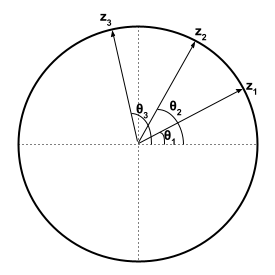
\includegraphics[width=0.5\textwidth]{figures/S1_Lie_group.png}
    \caption{S$_1$ group as Lie group.}
\end{figure}

This preserves the continuity of symmetry, so S$^1$ is smooth. 
Also, due to definition of multiplication and inversion, both the group operation of multiplication and inversion are also manifold.
This makes the group S$^1$ a Lie group. Moreover, the group operations are commutative, so the Lie group is \textbf{Abelian}.

\subsubsection{Lie Algebra}
An algebra, A over a field is a vector space over $\mathbb{C}$ equipped with bilinear product * defined as *:A $\times$ A $\rightarrow$ A.
Algebra is defined over a field implies that the vector space is also equipped with addition, multiplication, and scalar multiplication from the field.
Typically, algebra follows scalar multiplication and distributivity while commutativity and associativity are optional.
Let $\alpha, \beta, \gamma \: \epsilon$ A and c $\epsilon \: \mathbb{C}$ then

i. c ($\alpha * \beta$) = (c $\alpha) * \beta$ = $\alpha * (c \: \beta$) \\
ii. $\alpha * (\beta + \gamma $) = ($\alpha * \beta) + (\alpha* \gamma $)

Similarly, Lie algebra $\mathcal{L}$ is an algebra with operator [ , ] defined as [ , ]:$\mathcal{L} \times \mathcal{L} \rightarrow \mathcal{L}$.
Besides general properties of an algebra, Lie algebra has two other properties:
$\forall \: \alpha, \beta, \gamma \: \epsilon \: \mathcal{L}$

i. \textbf{skew-symmetry: } [$\alpha, \beta$] = - [$\beta, \alpha$] and [$\alpha, \alpha$] = 0 \\
ii. \textbf{Jacobi identity: } [$\alpha$, [$\beta, \gamma$]] + [$\beta$, [$\gamma, \alpha$]] + [$\gamma$, [$\alpha, \beta$]] = 0

These two properties are similar to vector multiplication.

\subsubsection{Exponential Map}
\href{https://en.wikipedia.org/wiki/Exponential_map_(Lie_theory)}{Exponential map} is a map from Lie algebra $\mathcal{L}$ of a Lie group \textbf{L} to the group, \textbf{exp:} $\mathcal{L} \rightarrow$ \textbf{L}, 
which allows one to recapture the local group structure from the Lie algebra. The ordinary exponential function is a special case of the exponential map when 
group G is the multiplicative group of positive real numbers (whose Lie algebra is the additive group of all real numbers).

The exponential of \textit{X} $\epsilon \: \mathcal{L}$ is denoted as \textbf{exp}(\textit{X}) and given by
\begin{equation}
    \textbf{exp}(X) = \sum_{k=0}^{\infty} \frac{X^k}{k!}
\end{equation}

If \textbf{L} be a \href{https://en.wikipedia.org/wiki/Lie_group#Matrix_Lie_groups}{matrix Lie group} then \textit{X} must have and inverse and det(\textit{X}) $\neq$ 0, so
there exists a matrix $\alpha$, logarithm of \textit{X} s.t.
\begin{equation}
    X = \textbf{exp}(\alpha) = \sum_{k=0}^{\infty} \frac{\alpha^k}{k!}
\end{equation}

The set of all matrices $\alpha$ whose exponentials belong to a group \textbf{L} is known as the Lie algebra, $\mathcal{L}$ of \textbf{L}.
Using the definition of the exponential series, we have
\begin{equation}
    X = \lim_{k \rightarrow \infty} \Big(I + \frac{\alpha}{k} \Big)^k \; \text{  and  } \; \alpha = \lim_{k \rightarrow \infty} k(X^{1/k}-I)
\end{equation}

For large k, the matrix (I + $\alpha$/k) is an operator of the group and gives \textit{X} by iteration. 
It is an \textbf{infinitesimal operator}, since for large k it differs from the identity operator by an infinitesimal amount.
Lie group is a manifold with a group structure and Lie algebra is its \textbf{tangent space}.
Elements of Lie algebra to a Lie group are sometimes referred to as \textbf{generators} of the group.
The Lie algebra can be thought of as the \textbf{infinitesimal vectors/operators} generating the group (at least locally) by means of
exponential map, but the Lie algebra doesn't form a generating set in strict sense.

\subsubsection{Generators of Lie Group}
Let $\alpha_j$ be a set of parameters the parameterize the Lie group \textbf{L} such that 
\begin{equation}
    \textit{g}(\alpha)|_{\alpha=0} = e
\end{equation}
where e is the identity element of Lie group \textbf{L}.

Let D be a representation of \textbf{L} then the linear operators of the representation will be parameterized the same way,
\begin{equation}
    D(\alpha)|_{\alpha=0} = I
\end{equation}
where I is the identity operator.

Then in some neighborhood of the identity element, we can Taylor expand D($\alpha$) as
\begin{equation}
    D(d\alpha) = 1 + i d\alpha_a X_a + ....
\end{equation}
where d$\alpha$ is infinitesimal and the sum over repeated indices should be understood as the "Einstein summation convention".

Then the generators of \textbf{L} are
\begin{equation}
    X_a = -i \frac{\partial D}{\partial \alpha_a}(\alpha)\Big|_{\alpha=0}
\end{equation}

In such a case,
\begin{equation}
    D(\alpha) = e^{iX_a\alpha^a}
\end{equation}

Why do we want to study Lie group through their generators? 
The truth is that the generators form an Algebra under \textbf{matrix commutation}. First of all, it is observed that the generators must all be operators in the same vector space 
the representation of the Lie Group maps to, so they must also form an operator vector space just like the group elements themselves. 
The only thing we need to check is that there exists a bilinear product in the vector space of the generators. 
The fact is that there is such a bilinear product called matrix commutator.

Let two group elements e$^{i\alpha^aX_a}$ and e$^{i\beta^bX_b}$, where $\alpha^a$ and $\beta^b$ are just two different set of
parameters for the Lie group, then by group closure,
\begin{equation}
    e^{i\alpha^aX_a} e^{i\beta^bX_b} = e^{i\delta^cX_c}
\end{equation}

Then we can write, 
\begin{equation}
    i\delta^cX_c = ln(e^{i\alpha^aX_a} e^{i\beta^bX_b}) = ln(1+ e^{i\alpha^aX_a} e^{i\beta^bX_b} -1) = ln(1+K)
    \label{eqn:lie_expansion}
\end{equation}

where \textit{K} = $e^{i\alpha^aX_a} e^{i\beta^bX_b} -1$

Then performing binomial expansion we finally get,
\begin{equation}
    i\delta^cX_c = i\alpha^aX_a + i\beta^bX_b - \alpha^aX_a \beta^bX_b - \frac{1}{2}\Big((\alpha^aX_a)^2-(\beta^bX_b)^2\Big) + \frac{1}{2}\Big(\alpha^aX_a + \beta^bX_b\Big)^2 + ....
\end{equation}
where the term 
\begin{equation}
    \Big((\alpha^aX_a)^2-(\beta^bX_b)^2\Big) + \Big(\alpha^aX_a + \beta^bX_b\Big)^2 = [\alpha^aX_a, \beta^bX_b]
\end{equation}
known as commutation operation.
No matter what the infinite sum in the right-hand side will be, it must be some linear combination of the generators multiply by \textit{i}.
Lets call it the linear combination $\gamma^c X_c$. Then,
\begin{equation}
    \begin{aligned}
        \relax [\alpha^aX_a, \beta^bX_b] = i\gamma^c X_c = i \alpha^a \beta^b f^c_{ab} X_c\\
       \implies [X_a, X_b] = i f^c_{ab} X_c 
    \end{aligned}
    \label{eqn:lie_bracket}
\end{equation}
The commutation relation \ref{eqn:lie_bracket} is called the Lie algebra of the group
which are completely determined by the constants $f^c_{ab}$ called the structural constants of the Lie Algebra. 
Even if we call them constants, $f^c_{ab}$ is really a three-tensor of constants.

We might wonder if we keep expanding \ref{eqn:lie_expansion} beyond second order, we would need additional conditions to make sure that the group multiplication law is maintained. 
The remarkable thing is that we don't. The commutator relation \ref{eqn:lie_bracket} is enough. 
In fact with structural constants $f^c_{ab}$ we can reconstruct as accurately as we like for any $\alpha$ and $\beta$ in some finite neighborhood of the origin. 
Thus the $f^c_{ab}$ are very important-they summarize virtually the entire group multiplication law.

For arbitrarily given $X_a$ , $X_b$ , $X_c$ , we can map from any two of the three generators to another one using matrix commutation. 
Thus, matrix commutator forms a bilinear product of the vector space of generators. 
The matrix commutators '[ , ]' are often called \textbf{Lie Bracket} in order to distinguish with another possible bilinear product for the generators \textbf{Poisson Bracket} '\{ , \}'.
In physics, Poisson Bracket is often used when we are working with classical Hamilton's equations. 
When the Poisson Bracket is replaced by Lie Bracket, it automatically implies the Hamiltonian or the Lagrangian is mapped to some Hilbert Space where the matrix
algebra works and the full Hamiltonian equation of motion reduces to the \textbf{Heisenberg picture} of quantum mechanics.

\subsubsection{SU(2) and SU(3) Groups}
Unit rotation in 2-dimension is the SO(2) group given by
\begin{equation}
    R(\theta) = \begin{pmatrix}
        cos\theta & -sin\theta \\ 
        sin\theta & cos\theta \\ 
\end{pmatrix}
\label{eqn:2d_R}
\end{equation}

However, a 3-dimensional representation of SO(2) is different from SO(3).
An SO(2) group in $\mathbb{R}^3$ is
\begin{equation}
    R(\theta) = \begin{pmatrix}
        1 & 0 & 0 \\ 
        0 & cos\theta & -sin\theta \\ 
        0 & sin\theta & cos\theta \\ 
\end{pmatrix}
\end{equation}

which is a unit rotation along the axis of unit vector (1, 0, 0) and this group doesn't represent akk 3D unit rotations.
There doesn't exist a 2D representation of a 3D rotation but there exists a 2D representation of some group whose algebra is the same as SO(3),
the group is called SU(2), which is defined in complex space.

To represent SO(2) using complex number we first define
\begin{equation}
    1 = \begin{pmatrix}
        1 & 0 \\ 
        0 & 1 \\ 
\end{pmatrix}, \;
i = \begin{pmatrix}
    0 & -1 \\ 
    1 & 0 \\ 
\end{pmatrix}
\end{equation}
then equation \ref{eqn:2d_R} can be represented as
\begin{equation}
    R(\theta) = cos\theta + sin\theta
\end{equation}

This equation forms a Lie group called U(1) where real number '1' is the generator of U(1) since
\begin{equation}
    e^{i*1\theta} = cos\theta + i sin\theta
\end{equation}

We can easily build a complex version of the SO(2) algebra because the entire symmetry group relies only on two degrees of freedom, 
so we can effectively use a single complex number to capture the dof. 
However, two dof is not enough for SO(3), so we consider higher dimension which leads us to U(2).
We can claim that only those unitary operators with determinant 1 will be sufficient to model the Algebra of SO(3) given that SO(3) has determinant 1 as well.
The unitary operators with determinant 1 are called \textbf{Special Unitary} operators and they form the group SU(2).
\begin{equation}
    SU(2) = \left\{
        \begin{pmatrix}
        \alpha & -\beta^* \\ 
        \beta & \alpha \\ 
    \end{pmatrix}: 
    \alpha, \beta \: \epsilon \: \mathbb{C}, |\alpha|^2+|\beta|^2=1
    \right\}
\end{equation}

The implication of the matrix elements of SU(2) in the usual two dimensional representation is that SU (2)
gives a maximum of four degrees of freedom, with two degree of freedom for each complex number. We then
need four basis operators to write all operators in SU(2). 
\begin{equation}
    1 = \begin{pmatrix}
        1 & 0 \\ 
        0 & 1 \\ 
    \end{pmatrix}, \;
    i = \begin{pmatrix}
        0 & i \\ 
        i & 0 \\ 
    \end{pmatrix}, \; 
    j = \begin{pmatrix}
        0 & 1 \\ 
        -1 & 0 \\ 
    \end{pmatrix}, \;
    k = \begin{pmatrix}
        i & 0 \\ 
        0 & -i \\ 
    \end{pmatrix}
\end{equation}

where $i^2 = j^2 = k^2 = -1$.
and every other element \textit{m} of SU(2) can be written as
\begin{equation}
    m = a + bi + cj + dk
\end{equation}
this is called \textbf{quaternion}.
We can then express our SO(3) basis operators $R_x(\theta)$, $R_y(\theta)$, and $R_z(\theta)$ as
\begin{equation}
    \begin{aligned}
        t_x(\theta) = cos(\theta) + sin(\theta) i \\
        t_y(\theta) = cos(\theta) + sin(\theta) j \\
        t_z(\theta) = cos(\theta) + sin(\theta) k
    \end{aligned}
\end{equation}

SU(2) is a dual cover of SO(3) which means we can map exactly two elements of SU(2) i.e. two $t$'s in SU(2) to one $R(\theta)$ in SO(3),
so if we consider a convex combination of $t_x$ , $t_y$ , and $t_z$, we span all elements of the entire SO(3).
We can examine the generators of the above 2D representation of SU(2):
\begin{equation}
    \begin{aligned}
        \sigma_x = -i \frac{dt_x}{d\theta}(0) = 
        -i \begin{pmatrix}
        -sin(0) & icos(0) \\ 
        icos(0) & -sin(0) \\ 
    \end{pmatrix} 
    \begin{pmatrix}
        0 & 1 \\ 
        1 & 0 \\ 
    \end{pmatrix} \\
    \sigma_y = -i \frac{dt_y}{d\theta}(0) = 
        -i \begin{pmatrix}
        -sin(0) & cos(0) \\ 
        -cos(0) & -sin(0) \\ 
    \end{pmatrix} 
    \begin{pmatrix}
        0 & -i \\ 
        i & 0 \\ 
    \end{pmatrix} \\
    \sigma_z = -i \frac{dt_z}{d\theta}(0) = 
        -i \begin{pmatrix}
        -sin(0) + icos(0) & 0\\ 
        0 & -sin(0) - icos(0) \\ 
    \end{pmatrix} 
    \begin{pmatrix}
        1 & 0 \\ 
        0 & -1 \\ 
    \end{pmatrix}
    \end{aligned}
\end{equation}
These are called \textbf{Pauli matrices} and for $i \neq j \neq k$
\begin{equation}
    [\sigma_i, \sigma_j] = 2i\epsilon_{ijk}\sigma_k
\end{equation}
Thus, the structural constants of SU(2) and SO(3) algebra must be the same. 

For example, the spin 1/2 representation is
\begin{equation}
    \begin{aligned}
        J^{1/2}_1 = \frac{1}{2}
    \begin{pmatrix}
        0 & 1 \\ 
        1 & 0 \\ 
    \end{pmatrix} = \frac{\sigma_1}{2}\\
    J^{1/2}_2 = \frac{1}{2}
    \begin{pmatrix}
        0 & -i \\ 
        i & 0 \\ 
    \end{pmatrix} = \frac{\sigma_2}{2}\\
    J^{1/2}_3 = \frac{1}{2}
    \begin{pmatrix}
        1 & 0 \\ 
        0 & -1 \\ 
    \end{pmatrix} = \frac{\sigma_3}{2}
    \end{aligned}
\end{equation}
The spin 1/2 representation is the simplest representation of SU(2). 
It is called the \textbf{defining representation} of SU(2), and is responsible for the name Special Unitary (SU).

\newpage
